% This is a sample document using the University of Minnesota, Morris, Computer Science
% Senior Seminar modification of the ACM sig-alternate style. Much of this content is taken
% directly from the ACM sample document illustrating the use of the sig-alternate class. Certain
% parts that we never use have been removed to simplify the example, and a few additional
% components have been added.

% See https://github.com/UMM-CSci/Senior_seminar_templates for more info and to make
% suggestions and corrections.

\documentclass{sig-alternate}
\usepackage{color}

%%%% User-defined macros
\newcommand{\lam}{\lambda}
\newcommand{\mycomment}[1]{\textcolor{red}{#1}}
%%%%% Uncomment the following line and comment out the previous one
%%%%% to remove all comments
%%%%% NOTE: comments still occupy a line even if invisible;
%%%%% Don't write them as a separate paragraph
%\newcommand{\mycomment}[1]{}

\begin{document}

% --- Author Metadata here ---
%%% REMEMBER TO CHANGE THE SEMESTER AND YEAR
\conferenceinfo{UMM CSci Senior Seminar Conference, April 2014}{Morris, MN}

\title{Interoperability in Programming Languages}

\numberofauthors{1}

\author{
% The command \alignauthor (no curly braces needed) should
% precede each author name, affiliation/snail-mail address and
% e-mail address. Additionally, tag each line of
% affiliation/address with \affaddr, and tag the
% e-mail address with \email.
\alignauthor
Todd Malone\\
	\affaddr{Division of Science and Mathematics}\\
	\affaddr{University of Minnesota, Morris}\\
	\affaddr{Morris, Minnesota, USA 56267}\\
	\email{malon153@morris.umn.edu}
}

\maketitle
\begin{abstract}
Interoperability of programming languages is the ability for two or more languages to interact as part of the same system. Frequently, this means passing messages and data between potentially very different languages.
The differences in these languages pose a serious barrier to creating an interoperative system.

However, interoperability is important to many existing systems today, as particular programming languages have emerged to target particular problem domains. In particular, client/server architecture and many distributed computing systems utilize multiple languages for differing parts of their system.


The problems inherent to cross language communication are myriad enough that no single approach could address all the issues, several such tools have emerged which approach the problems from different directions.
Two broad categories of these tools are virtual machines and markup languages. These two tools are used concurrently in many systems today, reflecting their different strengths.
\end{abstract}

\keywords{interoperability, language interoperability, programming languages, virtual machines, markup languages}

\section{Introduction}
Interoperability, colloquially shortened to interop, is the ability for two or more systems to work together. This definition is very broad, covering anything from groups of people to businesses or bureaucratic systems to pieces of hardware. This paper will discuss interoperability between programming languages. While this narrows the field significantly, programming language interop is still a very broad topic.

For instance, web browsers frequently perform some kind of interop. Information to be displayed on a web page is handled by a browser's interpretation of HTML, while any real-time aspect of the page will be handled by a language like JavaScript, again run from within the browser. If there is more computation to be done, or if a database needs to be consulted, the client, the browser, will communicate with a server, often written in languages like Java or C.

Likewise, these servers may be written in several languages themselves. A blog hosting service, Kidblog\footnote{kidblog.org}, uses a server written in both Java and Clojure, where Java handles translation between the client and server while Clojure handles the server-side logic.

The challenges that arise when dealing with interoperability can be many, and sometimes surprising \cite{Chisnall:2013}. The tools and approaches used to overcome these challenges are likewise many. In the interest of brevity, we will look at a small subset of these challenges, along with several tools used to deal with them.

In Section \ref{Interop} I explore further why interoperability is desirable, what advantages it can confer, and where it can be useful. This will touch on differing language capabilities, ease of use, hardware independence, and implications for distributed computing.

Next, in Sections \ref{VM} and \ref{ML}, I describe two particular tools that are commonly used to achieve interoperability. These tools will be virtual machines, paying particular attention to the Java Virtual Maching (JVM) and .NET's Common Language Runtime (CLR), and markup languages, with focus on two particular systems that make use of markup languages, Starlink and FML.

Section \ref{approaches} will detail particular challenges involved with interoperability and approaches to handling them. Following a general description of the approach, I will describe how each tool can be used to implement that approach, along with strengths and weaknesses of each setting.

Section \ref{performance} will look at a few of the performance implications of the tools discussed.


\section{Interoperability}\label{Interop}
The primary importance of interoperability lies in the varying capabilities of different languages. Programming languages are optimized for particular tasks, and different languages perform better in different situations.

Some languages are constructed to tackled specific problems, but provide reduced support for others. Erlang, for instance, is one of the primary languages used in distributed computing. It was built to handle remote procedure calls (RPCs), and does so simply and powerfully. However, intensive string manipulation in Erlang can be a challenge: Strings are not first class types in Erlang, nor do they even have a distinct type~\cite{ErlangTypeDoc}. Strings in Erlang are treated as character arrays, and while there is a module for string manipulation, it is significantly more light-weight than the Java or Ruby string classes. \mycomment{I'm considering removing reference to Java/Ruby here.}

Still others allow access in ways that are hidden in other languages. The memory access model in C, for instance, differs from many other high-level languages presently in use. C enables very fine-grained memory access and control, and places all of this control in the programmer's hands. Likewise, assembly languages allow direct access to hardware and the underlying storage mechanisms. This low-level control can be useful when dealing with systems with minimal memory, where the highest possible memory efficiency is required, or when access to device drivers is needed, for things like GPU computation.  However, these languages have high learning curves, and programs using them may have security concerns if not done correctly.

The difficulty involved in learning a language is not a minor concern, either. Developer time and energy are important considerations when designing a system.
This comes up particularly in systems involving legacy code. Say we have a system built in COBAL, which we want to build a web-based interface for. A distinct possibility with older systems is that the original developers are no longer on staff, and the new team is unfamiliar with both the code base and the language itself. In such a case, it may be faster or less expensive to have the developers create a bridge to the old system in a language they already know, and build the web interface to interact with the bridge. 


Apart from the capabilities of the languages involved, interoperability is often tied to hardware independence. The problems faced in achieving language independence and hardware independence are frequently similar, or have similar solutions. For instance, fuzzy controllers, which in part translate real-world input to fuzzy sets, are often strictly tied to the hardware they will be implemented upon. FML, the Fuzzy Markup Language, was developed as a way to fully describe such a controller in a hardware-independent manner. Part of this hardware independence involves independence from any particular implementing language; as such, a fuzzy controller specified in FML is capable of being implemented in or potentially across several different languages.~\cite{Acampora:2013}

In client/server architecture, such as in Kidblog, the client-side and server-side environments are likely written in different languages, and guaranteed to be on different machines. Kidblog handles communication between the two using JSON. On the client-side, JavaScript marshals blog posts into JSON objects, which are then sent to the server. There, they are converted to Java objects, which Clojure can then act on. Since Java is more strongly typed than JavaScript, JSON is also used to help translate between the two. We'll take a closer look at this in Section \ref{metadata}.



\section{Virtual Machines}\label{VM}
\begin{figure}
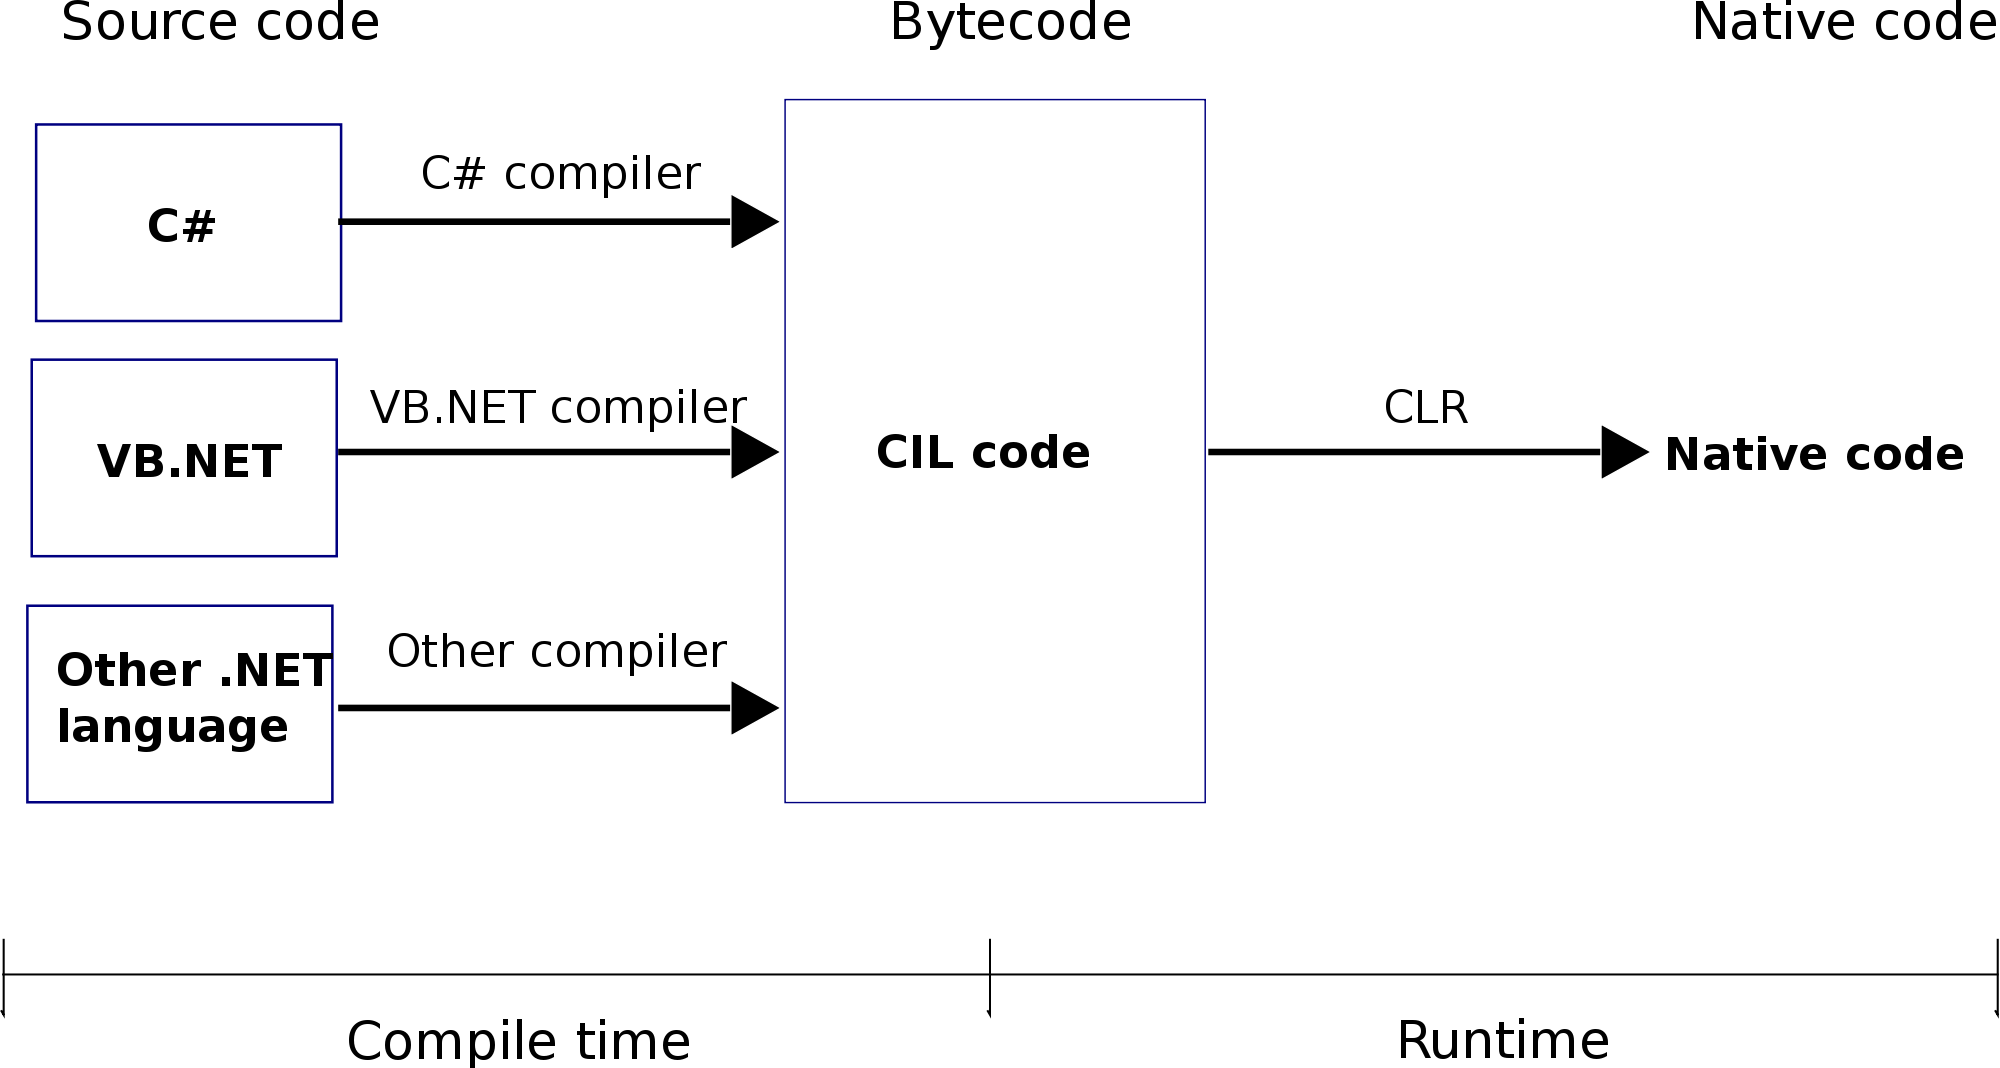
\psfig{file=CLR.png, width = 3in}
\caption{VM architecture in the CLR~\cite{wiki:CLR}}
\label{VMmodel}
\end{figure}

The term virtual machine (VM) refers to software that models the operating system of a computer or the underlying physical hardware. Effectively, VMs are indistinguishable from the OS or hardware they are emulating, which allows them to run programs not runable by the native OS, or with restrictions not enforced by the native OS or hardware.
The focus of this paper will be on virtual machines that act as a runtime environment for a single process, sometimes called process VMs. These VMs in particular enforce restrictions on what system resources their hosted process has access to. Specifically, they typically provide restricted, VM managed memory spaces, ensuring that hosted processes cannot access memory beyond what is allocated to it.~\cite{wiki:VM} \mycomment{is this relevant?}

There are two major advantages to virtual machines. The first of these is a type safety mechanism. Virtual machines such as the Java Virtual Machine (JVM) and .NET's Common Language Runtime (CLR) have a base set of types (in the CLR, this is actually called the Common Type System, or CTS. It is implicit and unnamed in the JVM). The VMs can use these type systems to ensure the correctness of participating languages and gives languages a common ground for their type information.

The second advantage lies in the VM's intermediate language. These are low-level languages, designed to be both compact and efficiently compiled to machine code, and are what is actually run by the virtual machine. As shown in Figure \ref{VMmodel}, any high-level language can be run on a virtual machine, as long as there is a compiler to translate that language into the VM's intermediate language.

These languages are still an abstraction of machine code, and so they still require an interpreter or a compiler for execution.
The VMs also contain interpreters for their intermediate language, but also utilize a run-time optimization method called Just-In-Time (JIT) compilation. Most of the code is still interpreted, but portions of code are monitored for frequent use. High-usage sections of code are compiled to machine language for quicker access. This allows for specific optimizations based on the current input and hardware, which are rarely known before execution.~\cite{wiki:JIT}



The JVM and CLR will be our main subjects when discussing virtual machines. While similar in certain ways, these two VMs were designed for different purposes.

The JVM\footnote{References to "The JVM" refer to the general concept of Java's virtual machine. There are many implementations of JVMs, which follow certain specifications but implement certain concepts in different ways and may support different operating systems.~\cite{wiki:multiJVM, wiki:JVM}}
was designed alongside Java for the purpose of hardware independence. Since the intent of Java was to be run off the web, there was no way of knowing what kind of hardware would end up running a piece of code, or even what kind of browser would be hosting that code. They needed to be able to compile to machine code only when the code was actually run, such that any hardware would be able to compile and run the code correctly. The solution was the JVM. The eventual discovery that other languages could make use of Java's intermediate language and the JVM was completely accidental.

In contrast, the CLR was developed to support a host of languages, and was designed in part with the intent of facilitating interoperability between them. The purpose of the virtual machine in this context was to intentionally provide the common ground for languages based on the CLR, giving them access to features promoting interop, such as the Common Type System and metadata engine (discussed further in Section \ref{metadata}).


\section{Markup Languages}\label{ML}
Markup languages (MLs) are primarily used for describing data. There are a range of markup languages covering several use cases, from document display or creation to data transfer and storage. For instance, HTML (HyperText Markup Language) is used to convey content information for web pages, while \TeX~is a language used to describe the layout and formatting of text documents.
Others, such as JSON and YAML, were designed for modeling data in ways consistent with object oriented design. JSON and YAML are not markup languages themselves, but 

One of the major players in the world of markup languages is XML, the Extensible Markup Language. XML's method of describing data is to enclose the relevant data with a tag. Tags are easily distinguishable from the data they contain, and are considered separate from the data when the XML is read. Notice in Figure \ref{MDL1} that the fields ({\tt Method, URI, Version}) are made distinct from the actual data with angled brackets.
Also note that tags can be nested: lines 11 through 14 are contained within the {\tt Header} tag. This allows XML to describe full records or objects, which will be important in Section \ref{metadata}.


\begin{figure}
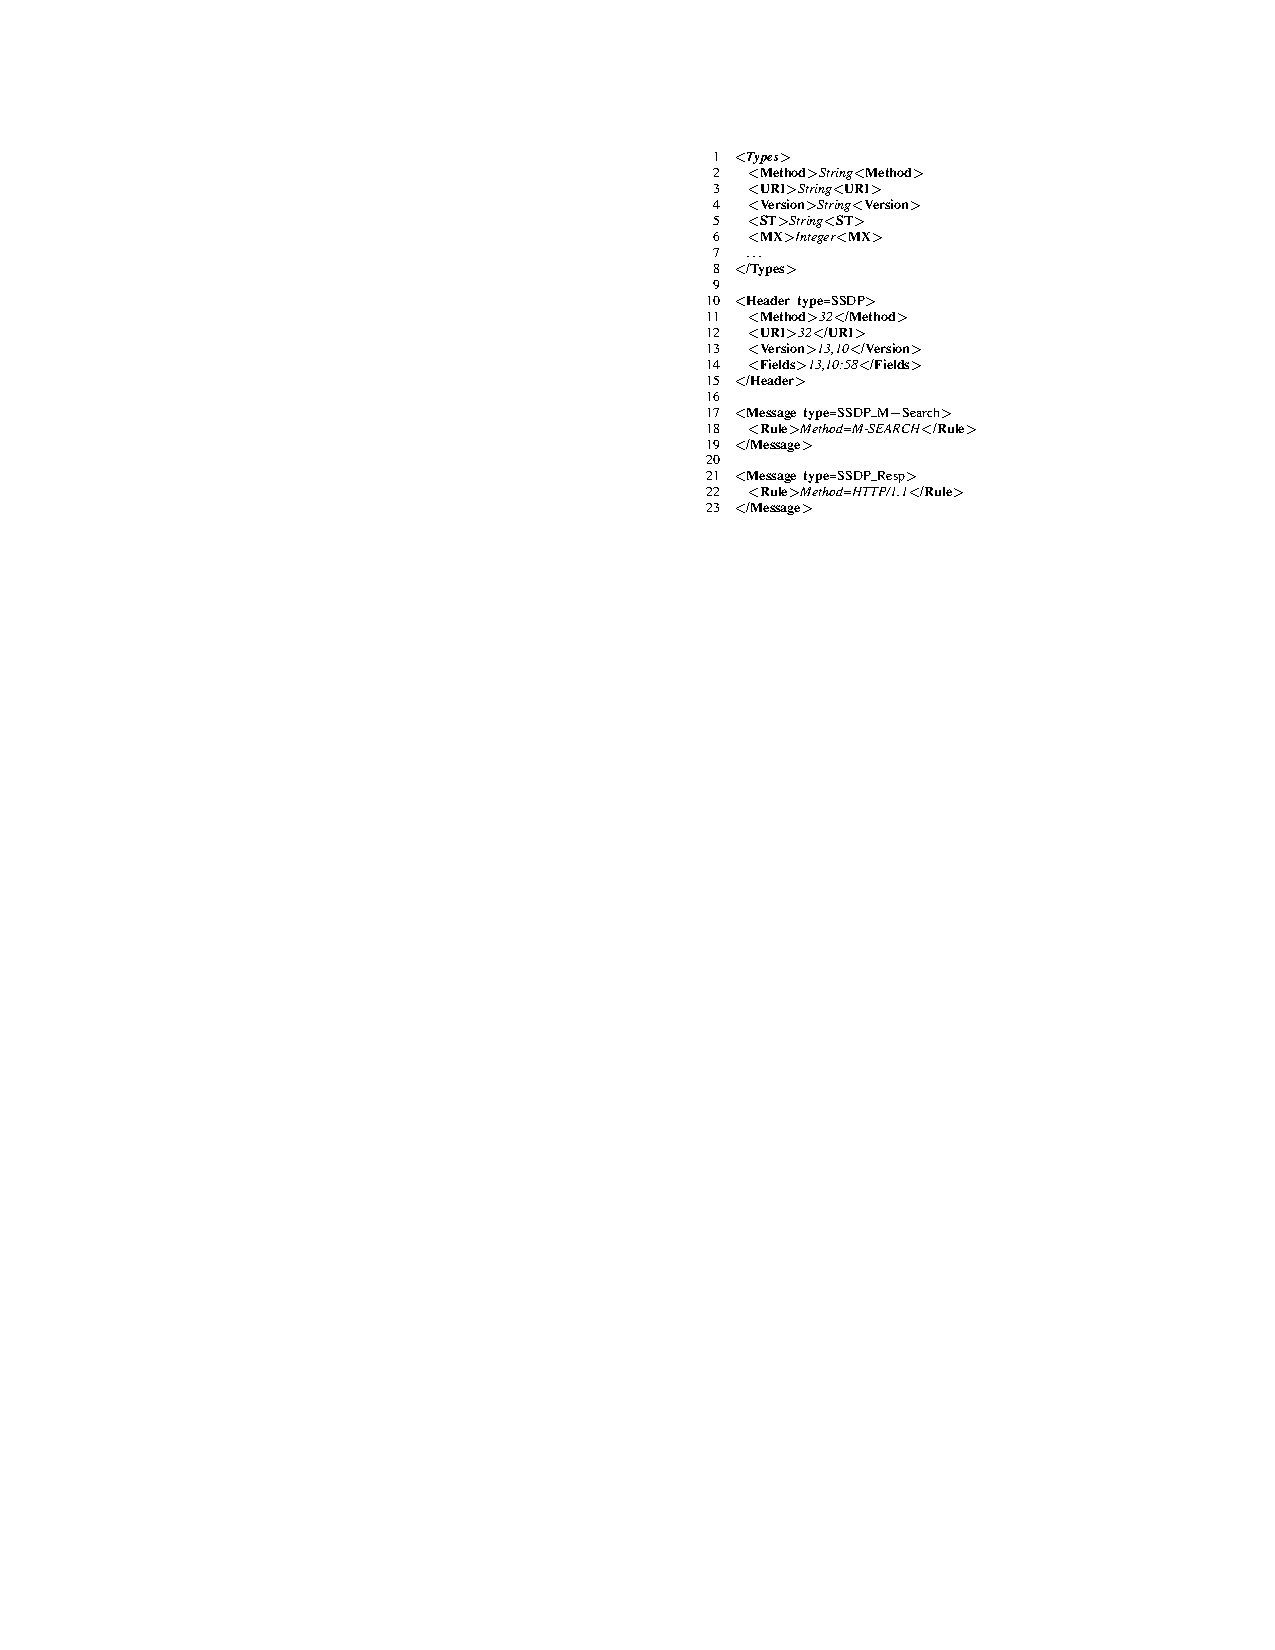
\psfig{file=StarlinkMDL.pdf}
\caption{A Starlink MDL specification (taken from~\cite{Bromberg:2011})}
\label{MDL1}
\end{figure}


The eponymous extensibility of XML comes in the form of defining new tags. Systems using XML are not constrained to using the tags built in to XML, but can create new ones based on the data they will be handling. This allows for the creation of new markup languages based on XML, but built for a specific purpose. HTML is one example of such a language. Two others, which we'll take a closer look at, are FML and Starlink.

Starlink~\cite{Bromberg:2011} is actually more than just a markup language. It is a software framework designed to achieve distributed interoperability between existing systems with different communications protocols. One of the core features of Starlink is XML-based markup languages called the Message Description Languages (MDLs). MDLs are used to model incoming messages from a protocol as abstract messages, which are network messages separated into their constituent parts and types. A translation logic specification, also written in XML, defines what parts in two MDLs can be related to one another. Once Starlink has performed appropriate transformations based on the message type received, it can then marshal a message for the target protocol using the newly created abstract message.

\section{Difficulties and Approaches}\label{approaches}
When building a system with interoperating languages, there are several aspects of the system that designers need to account for. Of particular importance is the lowest common denominator (LCD) constraint.

The LCD in this case is the largest subset of concepts that can be translated across the languages in use. These concepts include data types and underlying data structures.
For example, consider a system where key/value map would be useful, but one of the languages involved only has support for arrays. This restriction is part of the system's LCD, and limits the functionality of the overall system. Here, this can be dealt with in several ways: Remove the restricting language from the system, remove the use of maps and just use arrays instead, or find ways to model maps as arrays. The first two options are rarely preferable. If a particular language is present in a system, it usually has a contribution not easily matched by any other language. Likewise, maps may be the ideal way to store the particular data being used, while arrays will be insufficient.

Finding a method of translating a concept from one language to the other is preferable, but may not always be possible, or as straightforward as in the above example. In some cases, achieving the translation can mean a loss of information or a loss of precision. C, for instance, has no concept of booleans. Zero is treated as false, while any other number is treated as true. When interoperating with a language that does use booleans, precision of booleans is lost. A number could be just a number, or it could be True. On C's end, information could be lost if a true/false test is made to determine if a variable contains a number, and act upon that number if it does. If C recives a True from another language, it may read it as one.

For issues like these, there are two concepts that help enable this translation with minimal loss: metadata and standards.
\subsection{Metadata and Data Type Conversion}\label{metadata}
When passing data between two languages, a system must have a way of ensuring that the type systems of its component languages are respected. Additionally, it must ensure that type information is not lost when data moves from a strongly typed language to a weakly typed language, so that information is available when the data moves the other way.

Metadata is the method by which this is accomplished~\cite{Ide:2010}. Simply put, metadata is data describing data.
This can be almost anything, as long as it conveys information beyond what the data can by itself. In the case of strongly-typed languages, the type information included as part of a variable declaration is a kind of metadata. In Figure \ref{typedExample}, for instance, we can tell that there is a difference between the {\tt height} and {\tt weight} fields, despite both fields being a number.


\subsubsection*{VMs and metadata}

\begin{figure}
\begin{verbatim}
Class Person
  string name = "Cliff"
  date dateOfBirth = 4/16/1978
  int height = 74
  double weight = 212
end
\end{verbatim}
\caption{A Person class strongly-typed language}
\label{typedExample}
\end{figure}

\begin{figure}
\begin{verbatim}
Class Person
  var name = "Cliff"
  var dateOfBirth = 4/16/1978
  var height = 74
  var weight = 212
end
\end{verbatim}
\caption{A Person class in an untyped language}
\label{untypedExample}
\end{figure}

\begin{figure}
\begin{verbatim}
Class Person
  var name = ["Cliff", "string"]
  var dateOfBirth = [4/16/1978, "date"]
  var height = [74, "int"]
  var weight = [212, "double"]
end
\end{verbatim}
\caption{An untyped Person class, with type metadata}
\label{untypedMeta}
\end{figure}




There are two primary ways virtual machines handle metadata: language type specifications and metadata files. Both of these are handled by a compiler at compile time.
Once the system has been compiled to the intermediate language, there should be no syntactic difference between the different parts, as they are now all the same language.

As mentioned above, the explicit type information in strongly-typed languages, like Java or C\# is a kind of metadata. This metadata is entirely for use by their compilers, to assist with translation to the intermediate language.
In weakly or dynamically typed languages like Ruby and Groovy, this metadata does not exist (Figure \ref{untypedExample}). Since these languages perform run-time type checks instead of at compilation time, significantly more code is generated by their compilers, and they cannot take advantage of the intermediate language's primitive type system (everything must be assumed to be an Object-type object)\footnote{While this does have performance implications~\cite{Li:2013}, they do not outweigh the gains from utilizing the VM}.
\mycomment{I need to confirm this is true for Groovy}

Compilers for both the JVM and CLR also generate metadata along side the intermediate code. The JVM stores this metadata in the same file as the code, while the CLR stores it in a separate file in the same location. This metadata is used by the run-time interpreter for type checking and to assist with JIT optimization, but can also be accessed by other tools. 

\subsubsection*{MLs and metadata}
Metadata is the strong point of markup languages, as they are designed around the same concept of describing data. Essentially, the fields in a markup language (tags, in the case of XML-based languages) act as metadata for the data they are attached to.

When translating into an object for another programming language, 

The real metadata in a markup language can be stored in many ways. In Starlink's MDLs, for example, the type information of fields is stored in a {\tt <type>} tag before the definition of the fields begins, as can be seen in Figure \ref{MDL1} \cite{Bromberg:2011}. In other cases, the type information is stored in-line with specifications for correct formatting, as in XML schema (discussed in Section \ref{standards}).


\begin{figure}
\begin{verbatim}
<Person>
  <name> Cliff </name>
  <birthdate> 4/16/1978 </birthdate>
  <height> 74 </height>
  <weight> 212 </weight>
</Person>
\end{verbatim}
\caption{An XML description of a person}
\label{XMLexample}
\end{figure}

\subsection{Standards and Interfaces}\label{standards}
Metadata is the core of successful interoperability. But if two systems attempting to communicate are expecting differently tagged data, they will still fail to interoperate. Metadata alone is not enough.

There are two aspects to standards. One is agreement on similar data types, the other is the reaction to or approach to handling those types once received. Ide and Pustejovsky~\cite{Ide:2010} refer to this difference as syntactic interoperability (agreement on data type and communication protocols) and semantic interoperability (the ability to act on data received in a way unsurprising to other components of a system).

Shetty and Vadivel~\cite{Shetty:2009} demonstrate an example of a failure in semantic interoperability even while retaining some (though not all) syntactic interoperability between Java and .NET (CLR languages) web services.
While they found several syntactic mismatches, such as the lack of unsigned numbers in Java, there were issues even where the systems supported the same types. In particular, Shetty and Vadivel noted that null values were handled in largely incompatible ways. When given an array with a null element, Java interpreted as a null object, and printed {\tt null} when that element was requested. In contrast, .NET interpreted the element as empty, and printed an empty string when the element was requested. 
Additionally, they found that precision of decimal, double, and float types differed between platforms. When asked to add and display 4.111111 and 8.999999, the Java client returned 12.999999 with full precision, while the .NET client returned 13. 


\subsubsection*{VMs and Standardization}
Although the above study found issues between virtual machines, systems run on homogeneous virtual machines architecture actually have an advantage. Systems on a virtual machine already have a standard implemented in the form of the intermediate language. Because the intermediate language has a full language specification, including both a type system and data interpretation behavior, it can act as a description for required behavior. Moreover, once a system has been compiled into the intermediate language, the behavior of the different components is constrained by that virtual machine's behavior.

This is not a perfect solution however, as it still requires that the high-level languages have conventions for accessing other high-level language components.
These conventions are tied to compilers at least, so grammar for calling other languages on a particular VM can be included as part of a new compiler specification without affecting other implementations of that language.

As an example of this, Java was not initially intended to run other languages, making calls to non-Java languages is a difficult proposition~\cite{Chisnall:2013}. However, new JVM languages, like Clojure and JRuby, inherently provide support for accessing Java classes. \mycomment{would this benefit from an explicit example?}


\subsubsection*{MLs and Standardization}
Standards are not inherent to markup languages, and there is no simple way to use them to enforce anything more than syntactic interop. While this is a shortcoming of markup languages, it is hardly the end of the world: syntactic interoperability can be achieved by explicit standards at the development level, though this requires that developers be particularly aware of their system's LCD.

Semantic interop is much easier to attain with markup languages. Although not built in, many markup languages have a notion of schema, which can be used to regulate correct formatting. Messages sent in the markup language can be checked against these schema to ensure both that they contain the right fields in the right places, as well as that those fields contain the correct type of data. As Figure \ref{XMLschema} shows, type metadata can be stored within the schema specifications.

It should be noted that schema and similar mechanisms are themselves simply a standard, and are not expressly enforced or singular. XML has several schema languages associated with it. Figure \ref{XMLschema} is an example of the W3C\footnote{World Wide Web Consortium} recommended standard.


\begin{figure}
\begin{verbatim}
<?xml version="1.0" encoding="utf-8"?>
<xs:schema elementFormDefault="qualified" xmlns:xs="http://www.w3.org/2001/XMLSchema">
  <xs:element name="Person">
    <xs:complexType>
      <xs:sequence>
        <xs:element name="name" type="xs:string" />
        <xs:element name="birthdate" type="xs:date" />
        <xs:element name="height" type="xs:double" />
        <xs:element name="weight" type="xs:double" />
      </xs:sequence>
    </xs:complexType>
  </xs:element>
</xs:schema>
\end{verbatim}
\caption{A W3C-style XML schema for the person in Figure \ref{XMLexample}.}
\label{XMLschema}
\end{figure}



\section{Performance} \label{performance}
Regardless of how the system is built or the interop implemented, an interoperating system will always accrue some overhead. The cost of translating from one language to another can have surprising impacts on efficiency. 

The main issue faced in virtual machines is the LCD constraint. Because all languages eventually end up running in the same language, care must be taken that higher-level languages can be reasonably translated to the intermediate.
Li, White, and Singer \cite{Li:2013} show that in the Java Virtual Machine, non-Java languages rely heavily on existing Java code libraries in order to mitigate performance difficulties. Additionally, they found that non-Java languages produced sequences of bytecode distinct from those produced from Java source code.
For dynamically-typed languages like Ruby, these sequences are significantly longer than bytecode from an equivalent Java class. Additionally, JRuby bytecode contains none of the built-in type operators, which are used to optimize performance. This has some performance and space implications when comparing JRuby and Java, although JRuby does still see benefits from JIT optimization.


While I am not aware of a similar study focusing on languages on the CLR, the CLR was designed both with interoperability in mind and with an awareness that dynamically-typed languages would be running on it. From these two points, it seems reasonable to assume that CIL bytecode and the CLR interpreter are designed to handle dynamic types more efficiently or concisely.


The primary concern for markup languages is in translation time. Because systems involving MLs usually also involve different languages at runtime, they also require translating between two or three languages during execution.

Bromberg et al's report on the Starlink framework, which handles three translations per message, showed a non-negligible time lapse between when the initial message was received by Starlink and when Starlink returned a reply to that protocol.
\mycomment{Is this still too vague?}

Ultimately, the performance costs of achieving interoperability must be weighed against the potential performance gains. In systems involving several specialized domains, or in systems utilizing diverse hardware, the gains can well out-weigh the costs.



\section{Conclusions}


Virtual machines and markup languages each have strengths and weaknesses in different use cases.

Virtual machines are much more feasible for systems being built from scratch, where all language decisions are in the hands of the developers. They may also be available to existing programs on a VM which a developer wishes to extend to a larger system; in this case, the extended system merely need be built on the same virtual machine, and it will be able to interoperate with the pre-existing software.

In comparison, markup languages are better suited to dealing with preexisting or legacy systems, where there is too much code to make rewriting a feasible option, or where parts of the source are simply unavailable, potentially due to working with a third-party software. Likewise, if the existing system cannot target a particular virtual machine, perhaps because a compiler from that language to that VM doesn't exist, recompiling the existing program is not feasible.

Additionally, markup languages have an advantage in distributed system environments, where they can be used in sending data over the network. This is particularly important in client/server architecture, where servers have few, if any, guarantees about the hardware or sometimes even the software being run by the clients. A markup language can act as an intermediary, providing the data in a language and hardware free way.


These two cases are not mutually exclusive, and can even be complementary. A real-world system is more likely to make use of both virtual machines and markup languages to cover relevant aspects of their system than to rely on just a single approach.







%\section{Acknowledgments}


% The following two commands are all you need in the
% initial runs of your .tex file to
% produce the bibliography for the citations in your paper.
\bibliographystyle{abbrv}
% sample_paper.bib is the name of the BibTex file containing the
% bibliography entries. Note that you *don't* include the .bib ending here.
\bibliography{bibliography}  
% You must have a proper ".bib" file
%  and remember to run:
% latex bibtex latex latex
% to resolve all references

\end{document}
